\section{Uživatelské rozhraní}
%%%%%%%%%%%%%%%%%%%%%%%%%%%%
\subsection{Rozložení záznamu}
Rozložení jednotlivých záznamů bylo upraveno v menu objektu, v záložce \emph{Page Layouts}. Tato úprava je potřeba, jinak se atributy v uživatelském rozhraní neobjeví. 

Na obrázku \ref{fig:LD_Customer_Page_Layout} je vidět nastavení rozložení objektu a na obrázku \ref{fig:LD_Customer_Record_Layout} je vidět finální forma záznamu.

Rozložení záznamů bylo provedeno tak, aby uživatel při vyplňování informací postupoval shora dolů a informace byly rozděleny do logických celků.
\begin{figure}[h!]
    \centering
    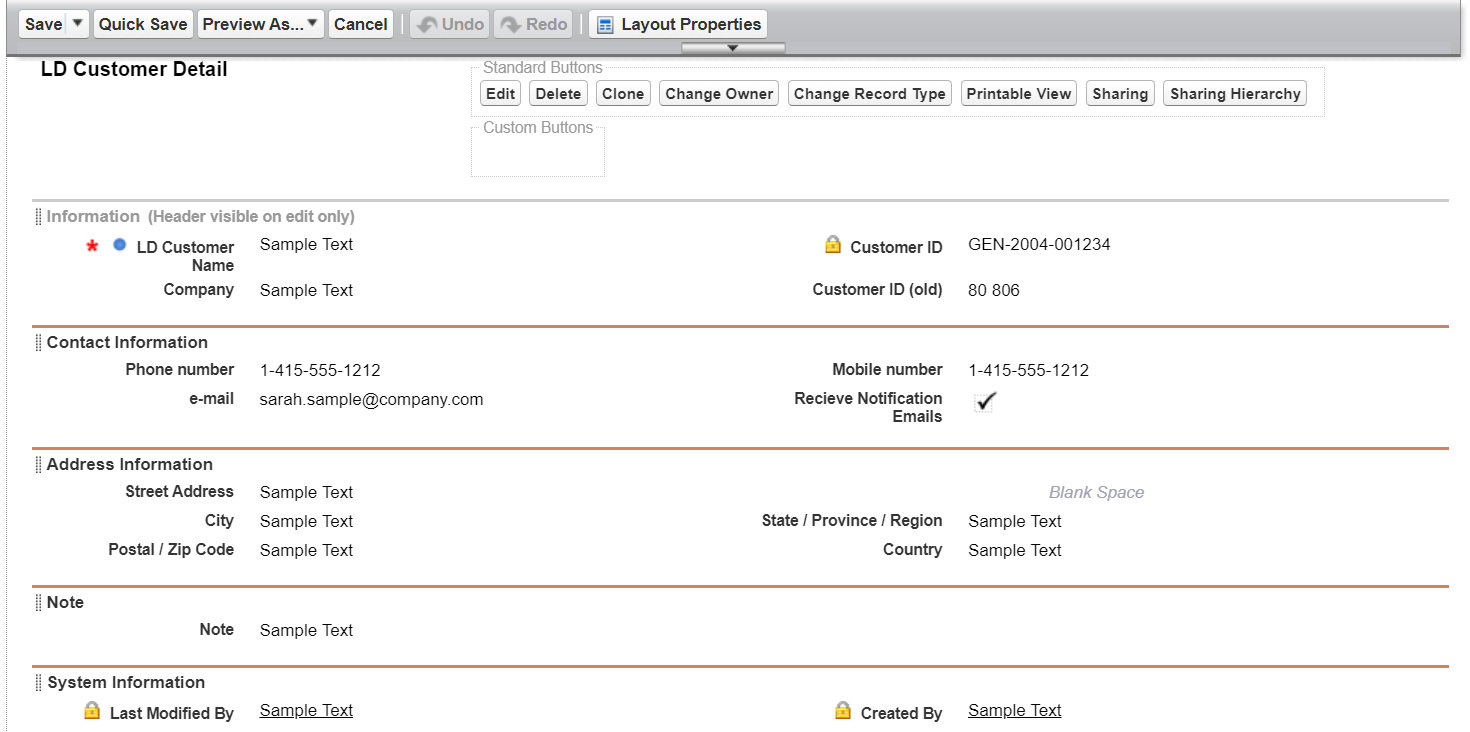
\includegraphics[width=\textwidth]{assets/7_implementace/uživatelské_rozhraní/LD Customer Page Layout.png}
    \caption{Nastavení Page Layout objektu LD Customer.}
    \label{fig:LD_Customer_Page_Layout}
\end{figure}
\begin{figure}[h!]
    \centering
    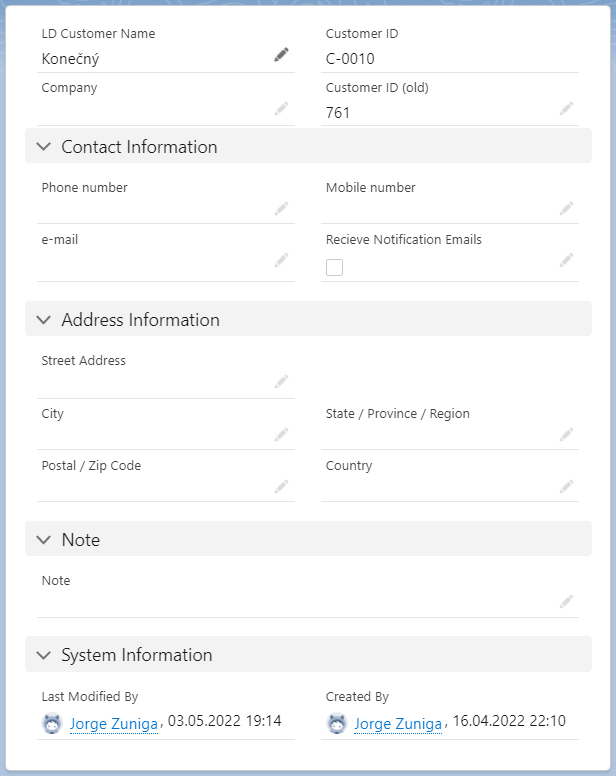
\includegraphics[width=0.6\textwidth]{assets/7_implementace/uživatelské_rozhraní/LD Customer Record Layout.png}
    \caption{Rozložení záznamu objektu LD Customer.}
    \label{fig:LD_Customer_Record_Layout}
\end{figure}
\FloatBarrier
%%%%%%%%%%%%%%%%%%%%%%%%%%%%
\subsection{Rozložení stránky záznamu}
Rozložení stránky záznamu je rozhraní, které se zobrazí po otevření jednotlivého záznamu. Rozložení stránky záznamu je k dispozici skrz menu nastavení v pravém horním rohu stránky. Po kliknutí na položku \emph{Edit Page} se otevře interaktivní editor stránky záznamu.
Editor rozložení stránky zákazníka je vidět na obrázku \ref{fig:LD_Customer_Page Builder}.

Rozložení stránek bylo provedeno tak, aby uživatel viděl co nejvíce informací o záznamu a nemusel otevírat jiné záznamy.
\begin{figure}[h!]
    \centering
    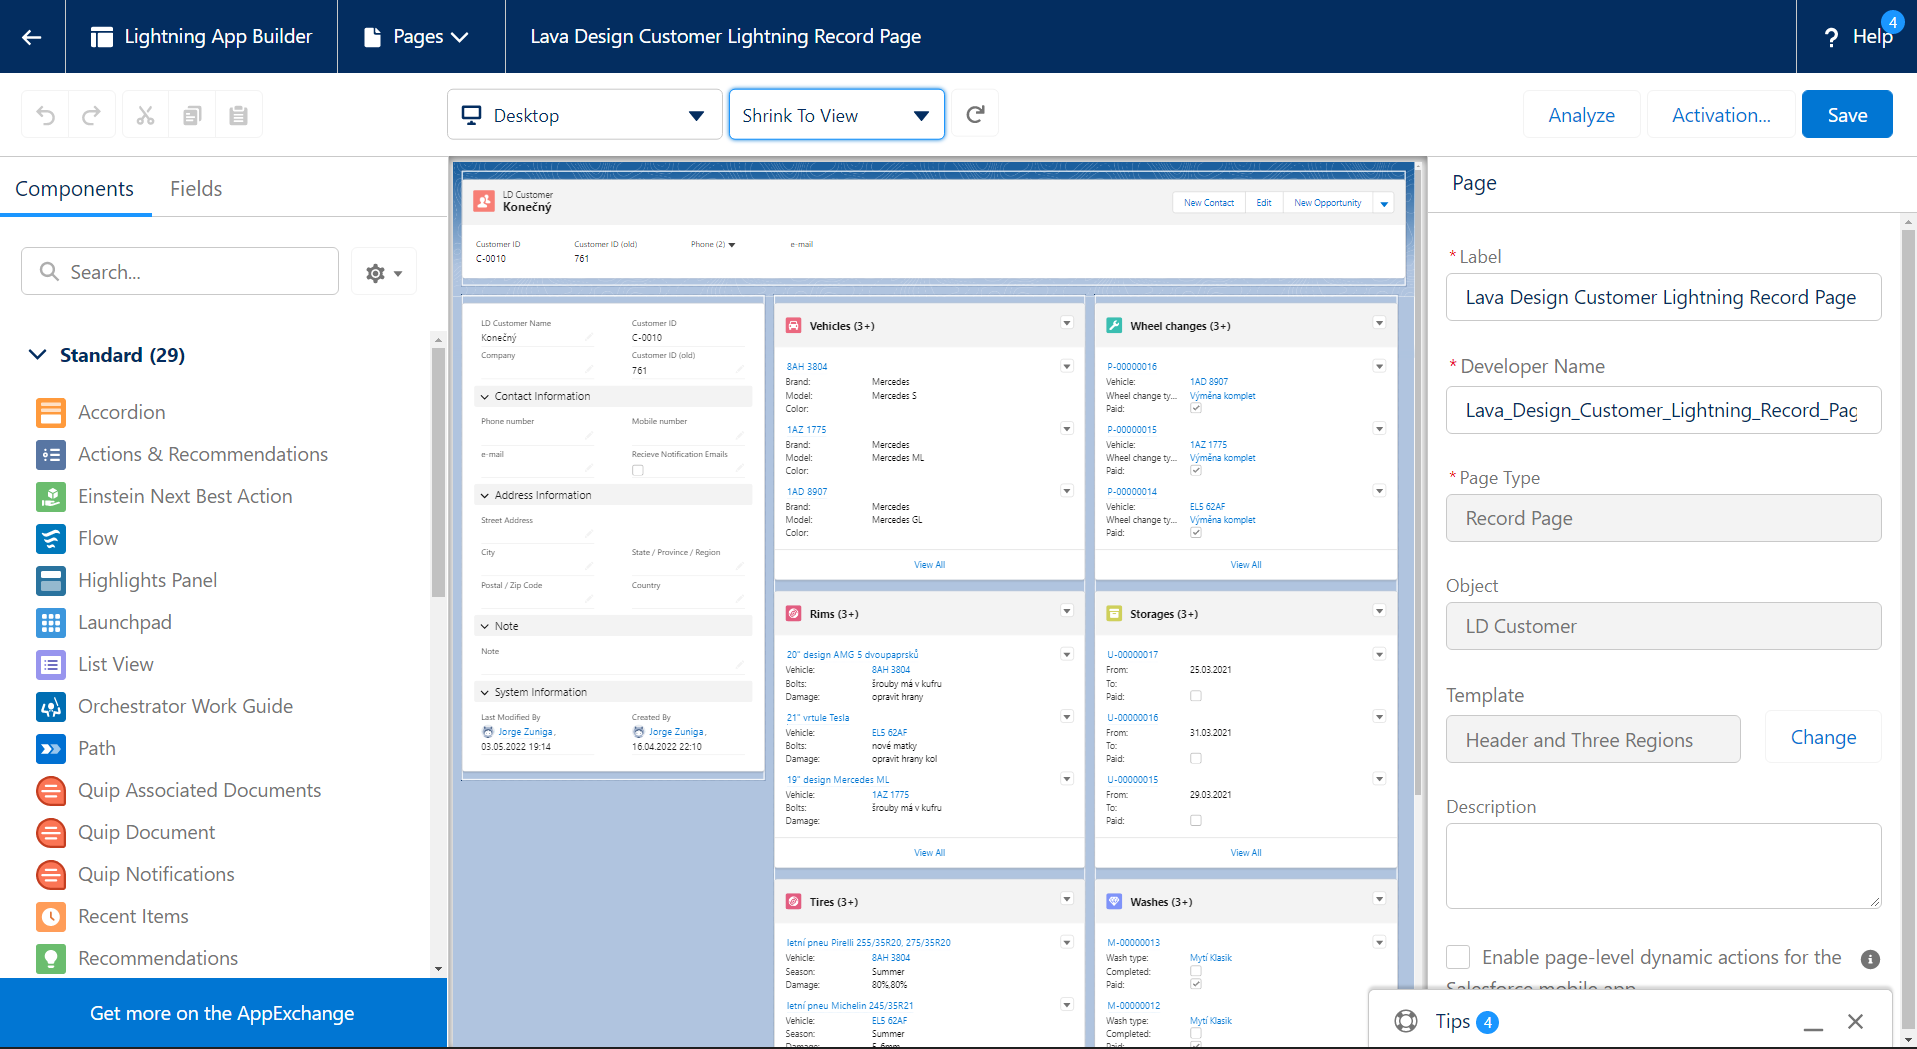
\includegraphics[width=\textwidth]{assets/7_implementace/uživatelské_rozhraní/Page builder - LD Customer.png}
    \caption{Editor stránky záznamu.}
    \label{fig:LD_Customer_Page Builder}
\end{figure}
\FloatBarrier
%%%%%%%%%%%%%%%%%%%%%%%%%%%%
\subsection{Kompaktní rozložení záznamu}
Kompaktní rozložení slouží k zobrazení informací o záznamu při přejetí myší, tím šetří potřebu otevírat nové záznamy.

Úprava kompaktního rozložení se provádí v menu objektu, v záložce \emph{Compact Layouts}. 

Kompaktní rozložení je vidět na obrázku \ref{fig:wheel_change_compact_layout}.
\begin{figure}[h!]
    \centering
    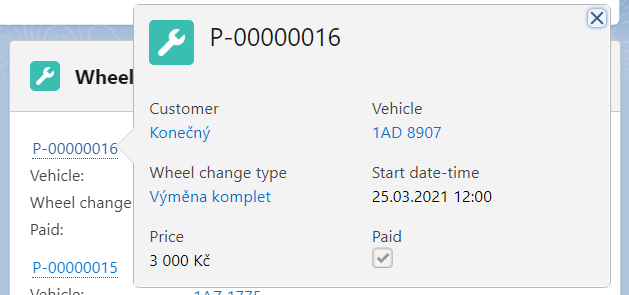
\includegraphics[width=0.8\textwidth]{assets/7_implementace/uživatelské_rozhraní/Wheel change detail.png}
    \caption{Kompaktní rozložení přezutí.}
    \label{fig:wheel_change_compact_layout}
\end{figure}
\FloatBarrier
%%%%%%%%%%%%%%%%%%%%%%%%%%%%
\subsection{Filtry záznamů}
V záložkách záznamů byly vytvořeny filtry. Příkladem je filtr: \emph{Neprovedené} u objektu oprav, který filtruje záznamy oprav, a zobrazí pouze ty, u kterých nebylo potvrzeno provedení. Výběr filtru je vidět na obrázku \ref{fig:record_filters}
\begin{figure}[h!]
    \centering
    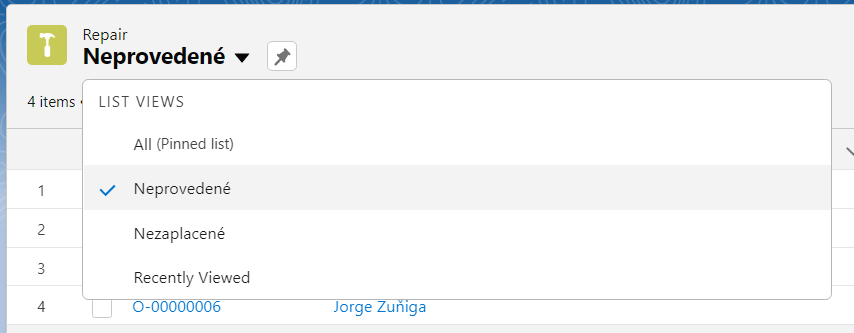
\includegraphics[width=\textwidth]{assets/7_implementace/uživatelské_rozhraní/Record filters.png}
    \caption{Filtry oprav.}
    \label{fig:record_filters}
\end{figure}
\FloatBarrier
%%%%%%%%%%%%%%%%%%%%%%%%%%%%
\subsection{Domovská stránka}
Domovská stránka je první stránka, která se zobrazí při otevření aplikace.

Editor rozložení domovské stránky je dostupný stejným způsobem jako editor rozložení záznamu.

Rozhraní domovské stránky bylo navrženo tak, aby majitel pneuservisu měl přehled o přezutích, která se ten den konají. Aby měl přehled o opravách a mytích, která ještě nejsou hotová. A aby měl k dispozici záznamy, u kterých nedávno byl, a mohl se k nim rychle vrátit.
\begin{figure}[h!]
    \centering
    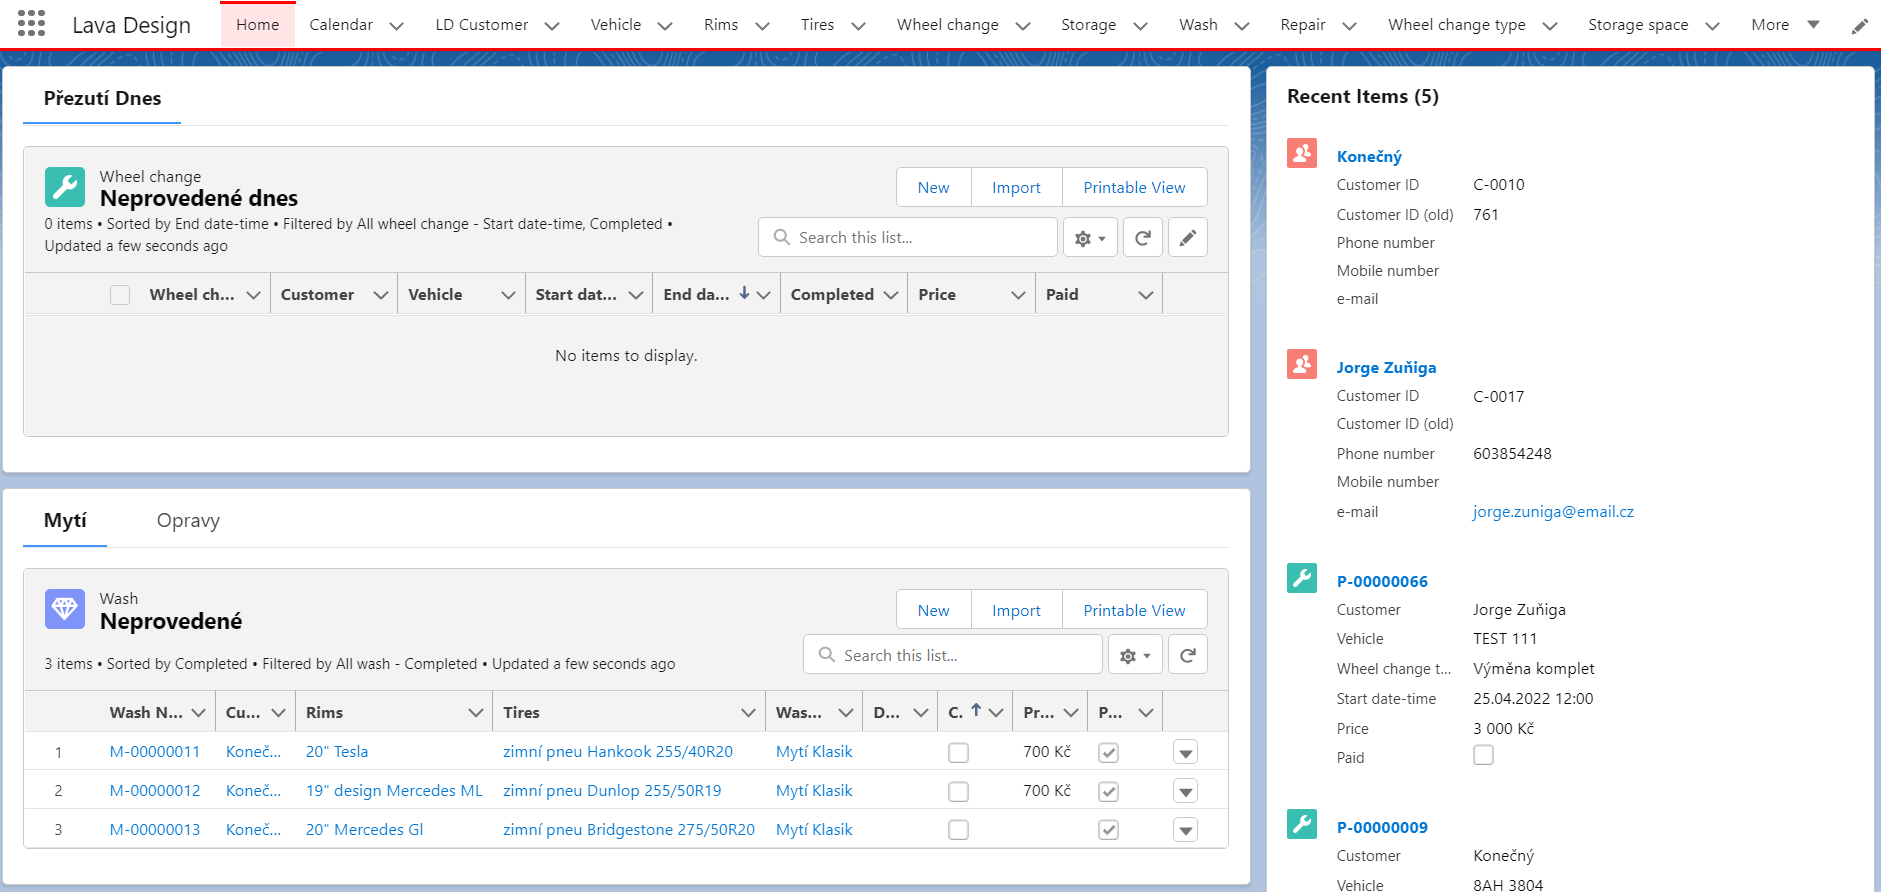
\includegraphics[width=\textwidth]{assets/7_implementace/uživatelské_rozhraní/Home page.png}
    \caption{Domovská stránka.}
    \label{fig:Home_page}
\end{figure}
\FloatBarrier
